\documentclass{article} % For LaTeX2e
\usepackage{nips13submit_e,times}
\usepackage{hyperref}
\usepackage{graphicx}
\usepackage{url}
\usepackage{CJK}
%\documentstyle[nips13submit_09,times,art10]{article} % For LaTeX 2.09

\title{RainbowNet:  Color Extrapolation from Grayscale Images}

\author{
Emily Ling\\
Computer Science\\
Stanford University\\
\texttt{eling8@stanford.edu} \\
\And
Cindy Lin \\
Computer Science\\
Stanford University\\
\texttt{cinlin@stanford.edu} \\
\And
Owen Wang \\
Computer Science\\
Stanford University\\
\texttt{ojwang@stanford.edu} \\
}

% The \author macro works with any number of authors. There are two commands
% used to separate the names and addresses of multiple authors: \And and \AND.
%
% Using \And between authors leaves it to \LaTeX{} to determine where to break
% the lines. Using \AND forces a linebreak at that point. So, if \LaTeX{}
% puts 3 of 4 authors names on the first line, and the last on the second
% line, try using \AND instead of \And before the third author name.

\newcommand{\fix}{\marginpar{FIX}}
\newcommand{\new}{\marginpar{NEW}}

\nipsfinalcopy % Uncomment for camera-ready version

\begin{document}

\maketitle

% report guidelines
% http://cs229.stanford.edu/cs229-final-report-guidelines.pdf

% [~1 paragraph]
\begin{abstract}

Inspired by digital recoloring of historical photos and Zhang et al.\cite{zhang}, our project aims to train a convolutional neural network to colorize black-and-white images, optionally augmenting with embeddings obtained from Google's Inception ResNet v2 (IRN2)\cite{resnet}. Given a batch of RGB images, we generate a possible colorization by training and predicting in the CIE Lab color space. We additionally analyze our training data to examine which distributions of colors most often occur together via K-clustering. Our model predicts mostly browns, blues, and reds and performed better without the added complexity of the IRN2 fusion.

\end{abstract}

% [~0.5 pages]
\section{Introduction}

Traditionally, the coloring of black-and-white historical photos is as much art as it is functional. Prints could take as long as a month to recolor as artists researched the colors on relevant fabrics, skin tones, and objects with the goal of bringing history back to life for contemporary viewers, who might otherwise feel detached from old black-and-white photographs. Groups such as ColorizedHistory\cite{reddit} bring together dozens of semi-professional colorizers for this task, and Time magazine has commissioned colorizers to produce a gallery of colored photographs of Abraham Lincoln in the hopes of creating a "vibrant documentation" of the historical figure.\cite{lincoln}\\

We would like to explore how well a deep learning approach performs on a task that takes human colorizers months to accomplish. With grayscale images as inputs, we use a convolutional neural network to output a predicted color per pixel. Our goal is to generate a plausible (and hopefully unique and interesting!) colorization to observers.

% [~0.5 pages]
\section{Related Work}

% TODO


% Describe your dataset: how many training/validation/test examples do you have? Is there any preprocessing you did? What about normalization or data augmentation? What is the resolution of your images? How is your time-series data discretized? Include a citation on where you obtained your dataset from. Depending on available space, show some examples from your dataset. You should also talk about the features you used. If you extracted features using Fourier transforms, word2vec, histogram of oriented gradients (HOG), PCA, ICA, etc. make sure to talk about it. Try to include examples of your data in the report (e.g. include an image, show a waveform, etc.).

% [0.5-1 pages]
\section{Dataset and Features}

\subsection{Lab Color Space}

For inputs into our CNN, we represent all images in the CIE Lab color space, which contains three channels: L for lightness and a and b for the color components green-red and blue-yellow. This allows for easy separation of black-and-white from color information, allowing us to use the L channel as input and ab channels as the desired output.\\

\subsection{ab Channel Discretization}

% TODO(eling8) - grid size of ???
We additionally discretize the ab space into 112 buckets and use bucket indices as the desired output instead of raw ab values during training. Our main motivation for this bucketing schema is due to the nature of loss functions based on distance between the predicted and true label. Because these functions are best minimized by mid-range values for a and b, minimizing the loss function does not provide the vibrancy in color we seek in our predictions. Furthermore, since the RGB color space is contained entirely within the CIE Lab color space, we may predict an Lab color that is outside of the possible set of RGB colors, giving an invalid result. Thus, we need some way of restricting the possible output set to only the CIE Lab colors that have a valid RGB mapping. Instead of directly predicting values for a, b, we divide the ab output space into buckets, and compute a probability distribution over the set of discrete colors. We chose to quantize the ab output space, where a and b each range from -128 to 127, into buckets with grid size of \textbf{[INSERT NUMBER HERE]}, excluding buckets that lie outside the RGB color space. This produced a total of 112 buckets. Using a set of discrete colors allows us to treat this problem as a multinomial classification problem, where for each pixel, we predict a probability distribution over the 112 buckets and use the bucket with the highest probability. These 112 buckets are plotted in CIE Lab color space in the figure below, with L=50:

\centerline{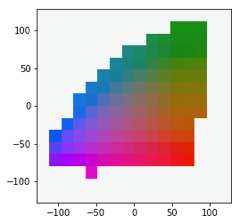
\includegraphics[scale=0.5]{112_buckets.png}}

\subsection{Preprocessing}

% TODO - missing x, y, z numbers
Our dataset contains 10K images from Unsplash\cite{dataset}, which are broken into \textbf{[INSERT NUMBER HERE]} training, \textbf{[INSERT NUMBER HERE]} validation, and \textbf{[INSERT NUMBER HERE]} test examples. The images are mostly 256x256 portraits and are preprocessed as follows:

% TODO - check for accuracy, esp re: normalization that might've been removed later
\begin{enumerate}
\item 256x256 RGB images resized to 224x224
\item RGB images converted to grayscale and fed into IRN2 to obtain an embedding per image
\item RGB images normalized to [0, 1] and converted to Lab color
\item Lab images separated into L and ab channels
\item L channel normalized to [0, 1]
\item ab channels discretized and represented by bucket index at each pixel
\end{enumerate}

As a result, we obtain the L channel (224, 244, 1) and IRN2 embeddings (1000,) as our inputs and the discretized ab channels (224, 224, 1) as the supervisory signal. Here are a few sample images from our training, validation, and test sets:\\

% TODO - insert a row of images, maybe 3 each?

% [1-1.5 pages]
\section{Methods}



% [1-3 pages for Experiments, Results, Discussion total]
\section{Experiments}

\section{Results}

\section{Discussion}

% [1-2 paragraphs]
\section{Conclusion and Future Work}

% WARNING: All sections before this point must fit on five (5) pages.

\section{Contributions}

% TODO(eling8)
\emph{Emily Ling}: color bucketing, data processing

\emph{Cindy Lin}: baseline, milestone writeup, customized colorization loss, K-clustering, final paper

% TODO(ojwang)
\emph{Owen Wang}: Rainbownet architecture, some debugging of loss and preprocessing

% note: please put bibitems in the order in which they are mentioned in the paper
\begin{thebibliography}{8}

\bibitem{zhang}
Zhang, R, Isola, P, Efros, A (2016). Colorful Image Colorization. University of California, Berkeley. Retrieved from https://arxiv.org/pdf/1603.08511.pdf.

\bibitem{resnet}
“Improving Inception and Image Classification in TensorFlow,” Research Blog, 31-Aug-2016. [Online]. Available: https:// research.googleblog.com/2016/08/improving-inception-and-image.html.

\bibitem{reddit}
“History in Color - ColorizedHistory,” reddit. [Online]. Available: https://www.reddit.com/r/ColorizedHistory/.

\bibitem{lincoln}
“Modernized President: Portraits of Abraham Lincoln, In Color,” Time. [Online]. Available: http://time.com/3792700/a-vibrant-past-colorizing-the-archives-of-history/.

\bibitem{dataset}
FloydHub - Deep Learning Platform - Cloud GPU. [Online]. Available: https://www.floydhub.com/emilwallner/datasets/colornet.

% milestone bibliography items
% \bibitem{7years}
% ronzohar (2016). Lukas Graham - 7 Years - Colored by an AI. Dailymotion. Retrieved from http://www.dailymotion.com/video/k4JjyaJtrPAOMziOYvH

% \bibitem{baldassarre}
% Blaldassarre, F., Morin, D.G., Rodes-Guirao, L. (2017). Image Colorization Using CNNs and Inception-Resnet-v2. KTH Royal Institue of Technology. Retrieved from https://github.com/baldassarreFe/deep-koalarization

\end{thebibliography}

\end{document}
